\documentclass[conf]{new-aiaa}
%\documentclass[journal]{new-aiaa} for journal papers
\usepackage[utf8]{inputenc}

\usepackage{graphicx}
\usepackage{amsmath}
\usepackage[version=4]{mhchem}
\usepackage{listings}
\usepackage{color}
\usepackage{siunitx}
\usepackage{longtable,tabularx}
\usepackage{subcaption}
\usepackage{cleveref}
\usepackage{appendix}
\usepackage{cancel}
\usepackage{csvsimple}
\setlength\LTleft{0pt}

\title{AE721 - Boundary Layer Theory \\ Assignment - 03}

\author{Ramkumar S. \footnote{SC22M007, M.Tech., Aerospace AFM }}
\affil{SC22M007, M.Tech. Aerospace - Aerodynamics and Flight Mechanics}


\definecolor{mygreen}{rgb}{0,0.6,0}
\definecolor{mygray}{rgb}{0.5,0.5,0.5}
\definecolor{mymauve}{rgb}{0.58,0,0.82}

\lstset{
  backgroundcolor=\color{white},   % choose the background color; you must add \usepackage{color} or \usepackage{xcolor}; should come as last argument
  basicstyle=\footnotesize,        % the size of the fonts that are used for the code
  breakatwhitespace=false,         % sets if automatic breaks should only happen at whitespace
  breaklines=true,                 % sets automatic line breaking
  captionpos=b,                    % sets the caption-position to bottom
  commentstyle=\color{mygreen},    % comment style
  deletekeywords={...},            % if you want to delete keywords from the given language
  escapeinside={\%*}{*)},          % if you want to add LaTeX within your code
  extendedchars=true,              % lets you use non-ASCII characters; for 8-bits encodings only, does not work with UTF-8
  firstnumber=0001,                % start line enumeration with line 1000
  frame=single,                    % adds a frame around the code
  keepspaces=true,                 % keeps spaces in text, useful for keeping indentation of code (possibly needs columns=flexible)
  keywordstyle=\color{blue},       % keyword style
  language=Octave,                 % the language of the code
  morekeywords={*,...},            % if you want to add more keywords to the set
  numbers=left,                    % where to put the line-numbers; possible values are (none, left, right)
  numbersep=5pt,                   % how far the line-numbers are from the code
  numberstyle=\tiny\color{mygray}, % the style that is used for the line-numbers
  rulecolor=\color{black},         % if not set, the frame-color may be changed on line-breaks within not-black text (e.g. comments (green here))
  showspaces=false,                % show spaces everywhere adding particular underscores; it overrides 'showstringspaces'
  showstringspaces=false,          % underline spaces within strings only
  showtabs=false,                  % show tabs within strings adding particular underscores
  stepnumber=2,                    % the step between two line-numbers. If it's 1, each line will be numbered
  stringstyle=\color{mymauve},     % string literal style
  tabsize=2,                       % sets default tabsize to 2 spaces
  % title=\lstname                 % show the filename of files included with \lstinputlisting; also try caption instead of title
}

\begin{document}

\maketitle

\begin{abstract}
    This is the report generated for the questions that were solved for the
    assignment 3.
\end{abstract}


\section{Question}

\begin{figure*}[!h]
    \center
    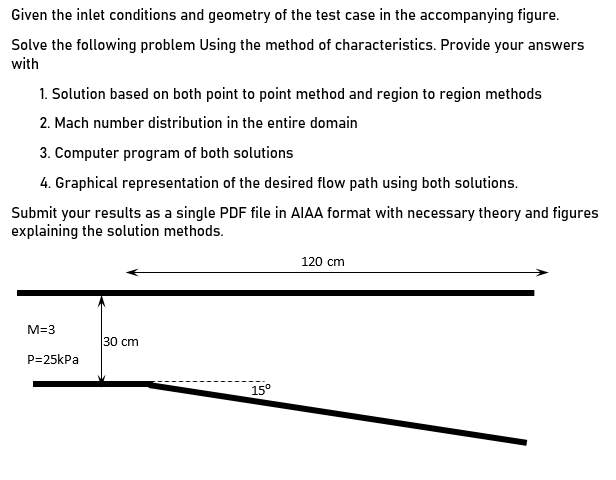
\includegraphics[scale=0.5]{results/question.png}
\end{figure*}

\textbf{SOLUTION:}\\

\par Given data
\begin{align*}
    M_1 &= 3.0 \\
    h &= 0.3 \ m \\
    L &= 1.2 \ m \\
    P_1 &= 25 \ kPa
\end{align*}

\par The solution algorithm followed for this problem is given below.\\

\par The number of characteristic nodes N, in the inlet plane is first chosen. The
value chosen for this problem is 100. An example layout of Characteristic lines
with N = 6, in the expansion flow domain of deflection angle $2^{\circ}$ is given in
\Cref{domain_layout}.But, the actual problem with $15^{\circ}$ deflection angle
requies N = 100 in order to accurately capture the expansion flow field. \\

\begin{figure}
   \center
    \includegraphics[scale=0.9]{results/expansion_corner_trial/char_map.png}
    \caption{Coarse characteristic points layout on the $2^{\circ}$ expansion corner}
    \label{domain_layout}
\end{figure}

\par Then the total number of characteristic nodes that will appear after all
interactions is computed using the equation below. Here, $n_{wall}$ is the number
of wall bounces requried as it is the one that controls the length of the
computation domain in this case. \\
\begin{align*}
    N_{total} = n_{wall} (2 N - 1) + N
\end{align*}

\par After this, a list of numbers indicating the characteristic points were
generated linearly similar to the one shown in \Cref{domain_layout} and the
points on both top and bottom wall is identified using the below equations
and were grouped for ease of computation.
\begin{align*}
    bottom\ wall: n_b = n_{b,prev} + (2N -1) \\
    top\ wall: n_b = n_{b,prev} + (N -1) \\
\end{align*}

\par Then a table, with the list of dependence upstream characteristic points,
to each internal and boundary char.point is made, which will be used during
computations. The inlet condition is defined such that, the expansion function
values $\nu(M)$ at all inlet char.points is computed for the following specified
condition. And the values of $K_1$ and $K_2$ were computed using the relations
given.
\begin{align*}
    M_{inlet} &= 3.0  \\
    \theta_{inlet} &= 0.0 \\
    K_1 &= \nu + \theta \\
    K_2 &= \nu - \theta
\end{align*}

\par Then the computation is begun for internal points, where the values of
$\nu$ and $\theta$ were computed by taking the intersected $K_1$ and $K_2$
upstream values as shown below.
\begin{align*}
    \nu &= \frac{K_1 + K_2}{2} \\
    \theta &= \frac{K_1 - K_2}{2}
\end{align*}

\par At the wall points, only one upstream characteristics meet, but the
wall angle $\theta_{wall}$ is known, hence using the upstream characteristic
and wall angle values, the expansion function is computed as shown in the
example below.
\begin{align*}
    bottom\ wall: \nu &= K_1 - \theta \\
    top\ wall: \nu &= K_2 + \theta
\end{align*}

\par Then, the Mach numbers at each characteristic point were computed using
Prandtl-Meyer expansion function relation given below.
\begin{align*}
    \nu(M) = \sqrt{\frac{\gamma+1}{\gamma-1}}tan^{-1}\sqrt{\frac{\gamma-1}{\gamma+1}\left(M^2-1\right)} - tan^{-1}\sqrt{M^2-1}
\end{align*}

\par For computing the location of downstream char.point, the following equations
that determine the slope of line (with the assumption that the char. curves are
straight lines in short length) and the location of the point as shown in the
\Cref{slope_image}.
\begin{figure}
    \center
    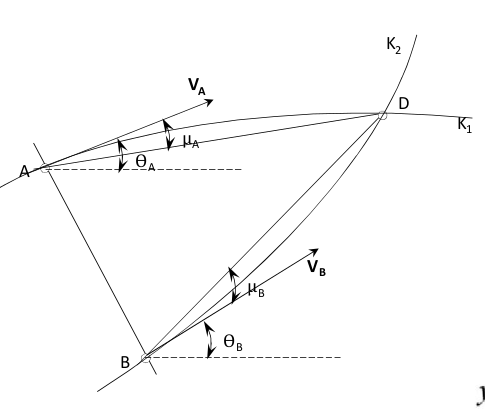
\includegraphics[scale=0.5]{results/slopeImage.png}
    \caption{reference image for the char. point position calculations}
    \label{slope_image}
\end{figure}


\begin{align*}
    \left(\frac{dy}{dx}\right)_A &= tan(\theta-\mu)_A \\
    \left(\frac{dy}{dx}\right)_B &= tan(\theta+\mu)_B \\
    S_1 &= \frac{tan(\theta-\mu)_A + tan(\theta-\mu)_B}{2} \\
    S_2 &= \frac{tan(\theta+\mu)_A + tan(\theta+\mu)_B}{2} \\
    y_D &=y_A + (x_D - x_A) S_1 \\
    y_D &=y_B + (x_D - x_B) S_2 \\
    x_D &= \frac{(S_2 x_B - S_1 x_A) + (y_A - y_B)}{S_2-S_1}
\end{align*}

\pagebreak
\textbf{Results:}

The Python code was developed for this computation and given in \Cref{appendixA}.
The contour of Mach number distribution and the characteristic points
obtained for this problem is given in \Cref{Mach_contour,char_output}, respectively. \\
\begin{figure}
    \center
    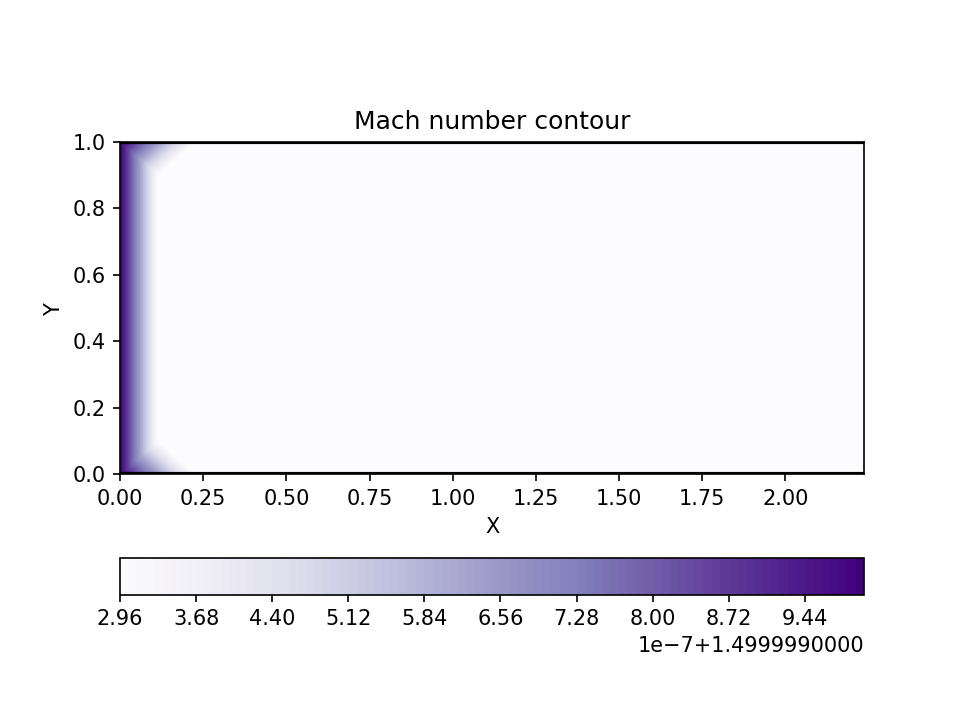
\includegraphics[scale=0.9]{results/expansion_corner/M_contour.png}
    \caption{Mach number contour output from computation}
    \label{Mach_contour}
\end{figure}

\begin{figure}
    \center
    \includegraphics[scale=0.9]{results/expansion_corner/char_map.png}
    \caption{characteristic points distribution (conjested due to 18k points for N = 100)}
    \label{char_output}
\end{figure}

\par Further, the Mach number of downstream section after expansion, obtained
from the computation is compared with the theoretical value obtained
from \cite{ref_1}. The following gives the values obtained and they found to
be in agreement with the theory.
\begin{align*}
    M_{2,computation} &= 3.92329 \\
    M_{2,theory} &= 3.923
\end{align*}

\pagebreak


\section{Question - 2}
Solve the Falkner-Skan equation numberically with appropriate boundary
conditions for \\ m = 2.0,1.0,0.6,0.3,0.0,-0.05,-0.08,-0.09043.

\vspace{0.5cm}
\textbf{SOLUTION}
\vspace{0.5cm}

\par The Falkner-Skan equation is again given in \Cref{FS_equation}.
\begin{align}
    f^{\prime\prime\prime} + \left(\frac{m+1}{2}\right) f f^{\prime\prime} + \left(1 - \left(f^{\prime}\right)^2\right) = 0 \label{FS_equation}
\end{align}

\par The appropriate boundary conditions are given below.

\begin{table*}[!h]
    \centering
    \begin{tabular}{cc}
        \underline{location} & \underline{conditions} \\
        $\eta = 0$ & $f = 0$ \& $f^{\prime} = 0$ \\
        $\eta = \infty$ & $f^{\prime} = 1$ \& $f^{\prime\prime} = 0$
    \end{tabular}
\end{table*}

\par It is a 3\textsuperscript{rd} order ordinary difference equation.
Hence to solve it numerically, the following two approaches have been followed.

\begin{enumerate}
    \item Finite-difference method
    \item Shooting method
\end{enumerate}

\subsection{Finite Difference Method}
\par In this method, following \cite{ref_1}, the \Cref{FS_equation} has split into
one 1\textsuperscript{st} order and one 2\textsuperscript{nd} order equations,
as given in \Cref{FD_eqn1,FD_eqn2}, this is done due to the limitation in the
boundary conditions available.
\begin{align}
    f^{\prime} &= z  \label{FD_eqn1} \\
    z^{\prime\prime} + \frac{m+1}{2} f z^{\prime} + m \left(1 - \left(z\right)^2\right) &= 0 \label{FD_eqn2}
\end{align}

\par Here, the \(\eta_{max} = 10\) i.e. finite domain is considered and the
boundary conditions for these equations will be
\begin{table*}[!h]
    \centering
    \begin{tabular}{cc}
        \underline{location} & \underline{conditions} \\
        $\eta = 0$ & $f = 0$ \& $z = 0$ \\
        $\eta = \infty$ & $z = 1$
    \end{tabular}
\end{table*}

\par Further, \Cref{FD_eqn1,FD_eqn2} are written in their difference forms using
2\textsuperscript{nd} order central difference scheme as given in
\Cref{diff_eqn1,diff_eqn2}.
\begin{align}
    \frac{f_{i+1} - f_i}{2\frac{\Delta \eta}{2}} &= \frac{1}{2}\left(z_i + z_{i+1}\right) \label{diff_eqn1}\\
    \frac{z_{i-1} -2 z_i + z_{i+1}}{\Delta \eta^2} + \left(\frac{m+1}{2}\right)f_i \frac{z_{i+1} - z_{i-1}}{2 \Delta \eta} + m \left(1 - z_i^2\right) &= 0 \label{diff_eqn2}
\end{align}

\par Then the \Cref{diff_eqn1,diff_eqn2} are rearranged to the forms which can be
programmed as given in \Cref{alg_eqn1,alg_eqn2}.
\begin{align}
    f_{i+1} &= f_i + \frac{1}{2}\left(z_i + z_{i+1}\right)\Delta\eta; i = 1,2,...,N-1 \label{alg_eqn1} \\
    a_i z_i &= b_i z_{i+1} + c_i z_{i-1} + d_i; i = 2,3,4,...,N-1 \label{alg_eqn2}
\end{align}

where
\begin{align*}
    a_i &= \left(\frac{2}{\Delta\eta^2} + m z_i\right) \\
    b_i &= \left(\frac{1}{\Delta\eta^2} + \frac{m+1}{4 \Delta \eta}f_i\right) \\
    c_i &= \left(\frac{1}{\Delta\eta^2} - \frac{m+1}{4 \Delta \eta}f_i\right) \\
    d_i &= m
\end{align*}

\par For each iteration, the \Cref{alg_eqn1} is marched forward from \(\eta = 0\)
till \(\eta = \eta_{max} = 10\) and the \Cref{alg_eqn2} is solved iteratively
till convergence.\\

The solution steps followed are given below.
\begin{enumerate}
    \item initialize \(z_i\) and \(f_i\)
    \item start outer iteration.
    \item solve \Cref{alg_eqn1} by marching forward in \(\eta\) direction.
    \item solve \Cref{alg_eqn2} iteratively using the values of \(f_i\) computed in previous step, till convergence.
    \item check for convergence using \(z_i\) values from previous and present outer iteration.
    \item continue outer iteration till convergence.\\
\end{enumerate}

\par The \Cref{FS_equation} is solved using this method for all m values except
\(m = -0.09043\), this method does not converge for this m value. Hence
the next, shooting method is used for \(m = -0.09043\).

\par The \emph{Python} code developed for this analysis is given in \Cref{FDM_code}

% shooting method--------------------------------------------------------------
\subsection{Shooting method}
\par In this method, the \Cref{FS_equation} is split into 3 1\textsuperscript{st}
order ODEs as given in \Cref{SH_eqn1,SH_eqn2,SH_eqn3}.

\begin{align}
    f^\prime &= g \label{SH_eqn1} \\
    g^\prime &= h \label{SH_eqn2} \\
    h^\prime &= -(1 - g^2) m - \left(\frac{m+1}{2}\right) f h \label{SH_eqn3}
\end{align}

\par Here also, the \(\eta_{max} = 10\) i.e. finite domain is considered and the
boundary conditions for these equations will be
\begin{table*}[!h]
    \centering
    \begin{tabular}{cc}
        \underline{location} & \underline{conditions} \\
        $\eta = 0$ & $f = 0$ \& $g = 0$ \\
        $\eta = \eta_{max}$ & $g = 1$
    \end{tabular}
\end{table*}

\par Here, it can be seen that the initial condition i.e. the value of $h$ at
\(\eta = 0\) is unknown, but the value of $g$ at \(\eta = \eta_{max}\) is known.
Hence by shooting method, the initial value of $h$ at \(\eta = 0\) is assumed
and the solution is proceeded till $\eta_{max}$.

\par Now, the value of $g$ at $\eta_{max}$ may not match with the boundary
conditions, hence their error difference is taken as the key for adjusting
the initial $h$ value using \emph{bisection} method. The solution of
\Cref{FS_equation} with \(m = -0.09043\) is computed using this method.

\par The \emph{Python} code developed for this analysis is given in \Cref{SH_code}

\subsection{Tables of final iteration values}
Here, the first deliverable as the tables of computed values of
parameters for each value of m are given in \Cref{table_m1,table_m2,table_m3,table_m4,table_m5,table_m6,table_m7,table_m8}

\begin{table}
    \parbox{0.45\linewidth}{
        \centering
        \caption{computed values for m = -0.05}
        \begin{tabular}{|c|c|c|c|}
            \hline
            $\eta$ & $f$ & $f^\prime$ & $f^{\prime\prime}$ \\ \hline
            0.0 & 0.0 & 0.0 & 0.21247 \\ \hline
            0.5 & 0.0276 & 0.11241 & 0.23689 \\ \hline
            1.0 & 0.11434 & 0.23623 & 0.25729 \\ \hline
            1.5 & 0.26521 & 0.36819 & 0.26852 \\ \hline
            2.0 & 0.48291 & 0.50238 & 0.26545 \\ \hline
            2.5 & 0.76662 & 0.63073 & 0.24491 \\ \hline
            3.0 & 1.1112 & 0.74456 & 0.20795 \\ \hline
            3.5 & 1.50756 & 0.83693 & 0.16049 \\ \hline
            4.0 & 1.944 & 0.90479 & 0.11145 \\ \hline
            4.5 & 2.40845 & 0.94952 & 0.06915 \\ \hline
            5.0 & 2.89043 & 0.97583 & 0.03815 \\ \hline
            5.5 & 3.38218 & 0.98959 & 0.01868 \\ \hline
            6.0 & 3.87879 & 0.99598 & 0.0081 \\ \hline
            6.5 & 4.37754 & 0.99861 & 0.00311 \\ \hline
            7.0 & 4.87713 & 0.99957 & 0.00106 \\ \hline
            7.5 & 5.37701 & 0.99988 & 0.00032 \\ \hline
            8.0 & 5.87697 & 0.99997 & 9e-05 \\ \hline
            8.5 & 6.37697 & 0.99999 & 2e-05 \\ \hline
            9.0 & 6.87696 & 1.0 & 0.0 \\ \hline
            9.5 & 7.37696 & 1.0 & 0.0 \\ \hline
            10.0 & 7.87696 & 1.0 & 0.0 \\ \hline
        \end{tabular}
        \label{table_m1}
    }
    \hfill
    \parbox{0.45\linewidth}{
        \centering
        \caption{computed values for m = -0.08}
        \begin{tabular}{|c|c|c|c|}
            \hline
            $\eta$ & $f$ & $f^\prime$ & $f^{\prime\prime}$ \\ \hline
            0.0 & 0.0 & 0.0 & 0.09964 \\ \hline
            0.5 & 0.01413 & 0.0598 & 0.13949 \\ \hline
            1.0 & 0.0631 & 0.13925 & 0.17783 \\ \hline
            1.5 & 0.15644 & 0.2369 & 0.21171 \\ \hline
            2.0 & 0.30252 & 0.34949 & 0.2367 \\ \hline
            2.5 & 0.50748 & 0.47128 & 0.24766 \\ \hline
            3.0 & 0.77399 & 0.59416 & 0.24056 \\ \hline
            3.5 & 1.10024 & 0.70872 & 0.21472 \\ \hline
            4.0 & 1.47987 & 0.80644 & 0.17429 \\ \hline
            4.5 & 1.90294 & 0.88196 & 0.12751 \\ \hline
            5.0 & 2.35794 & 0.93442 & 0.08349 \\ \hline
            5.5 & 2.83402 & 0.967 & 0.04871 \\ \hline
            6.0 & 3.32251 & 0.98502 & 0.02525 \\ \hline
            6.5 & 3.81751 & 0.99388 & 0.01162 \\ \hline
            7.0 & 4.31557 & 0.99776 & 0.00475 \\ \hline
            7.5 & 4.81488 & 0.99926 & 0.00172 \\ \hline
            8.0 & 5.31467 & 0.99978 & 0.00056 \\ \hline
            8.5 & 5.81461 & 0.99994 & 0.00016 \\ \hline
            9.0 & 6.31459 & 0.99999 & 4e-05 \\ \hline
            9.5 & 6.81459 & 1.0 & 1e-05 \\ \hline
            10.0 & 7.31459 & 1.0 & 0.0 \\ \hline
        \end{tabular}
        \label{table_m2}
    }
\end{table}

\begin{table}
    \parbox{0.45\linewidth}{
        \centering
        \caption{computed values for m = 0.3}
        \begin{tabular}{|c|c|c|c|}
            \hline
            $\eta$ & $f$ & $f^\prime$ & $f^{\prime\prime}$ \\ \hline
                0.0 & 0.0 & 0.0 & 0.72548 \\ \hline
                0.5 & 0.0844 & 0.32522 & 0.57542 \\ \hline
                1.0 & 0.3127 & 0.57579 & 0.42788 \\ \hline
                1.5 & 0.64821 & 0.75504 & 0.29212 \\ \hline
                2.0 & 1.05724 & 0.87179 & 0.17972 \\ \hline
                2.5 & 1.51184 & 0.93989 & 0.09815 \\ \hline
                3.0 & 1.99162 & 0.975 & 0.04704 \\ \hline
                3.5 & 2.48364 & 0.99085 & 0.01962 \\ \hline
                4.0 & 2.98087 & 0.99707 & 0.00709 \\ \hline
                4.5 & 3.48004 & 0.99918 & 0.00221 \\ \hline
                5.0 & 3.97982 & 0.9998 & 0.00059 \\ \hline
                5.5 & 4.47976 & 0.99996 & 0.00014 \\ \hline
                6.0 & 4.97975 & 0.99999 & 3e-05 \\ \hline
                6.5 & 5.47975 & 1.0 & 0.0 \\ \hline
                7.0 & 5.97975 & 1.0 & 0.0 \\ \hline
                7.5 & 6.47975 & 1.0 & 0.0 \\ \hline
                8.0 & 6.97975 & 1.0 & 0.0 \\ \hline
                8.5 & 7.47975 & 1.0 & 0.0 \\ \hline
                9.0 & 7.97975 & 1.0 & 0.0 \\ \hline
                9.5 & 8.47975 & 1.0 & 0.0 \\ \hline
                10.0 & 8.97975 & 1.0 & 0.0 \\ \hline
        \end{tabular}
        \label{table_m3}
    }
    \hfill
    \parbox{0.45\linewidth}{
        \centering
        \caption{computed values for m = 0.6}
        \begin{tabular}{|c|c|c|c|}
            \hline
            $\eta$ & $f$ & $f^\prime$ & $f^{\prime\prime}$ \\ \hline
            0.0 & 0.0 & 0.0 & 0.97514 \\ \hline
            0.5 & 0.10943 & 0.41353 & 0.68262 \\ \hline
            1.0 & 0.39034 & 0.68916 & 0.42917 \\ \hline
            1.5 & 0.77986 & 0.85319 & 0.23864 \\ \hline
            2.0 & 1.23045 & 0.93904 & 0.1156 \\ \hline
            2.5 & 1.7111 & 0.97801 & 0.04815 \\ \hline
            3.0 & 2.20452 & 0.99317 & 0.01707 \\ \hline
            3.5 & 2.70261 & 0.99819 & 0.00511 \\ \hline
            4.0 & 3.20213 & 0.99959 & 0.00128 \\ \hline
            4.5 & 3.70203 & 0.99992 & 0.00027 \\ \hline
            5.0 & 4.20202 & 0.99999 & 5e-05 \\ \hline
            5.5 & 4.70201 & 1.0 & 1e-05 \\ \hline
            6.0 & 5.20201 & 1.0 & 0.0 \\ \hline
            6.5 & 5.70201 & 1.0 & 0.0 \\ \hline
            7.0 & 6.20201 & 1.0 & 0.0 \\ \hline
            7.5 & 6.70201 & 1.0 & 0.0 \\ \hline
            8.0 & 7.20201 & 1.0 & 0.0 \\ \hline
            8.5 & 7.70201 & 1.0 & 0.0 \\ \hline
            9.0 & 8.20201 & 1.0 & 0.0 \\ \hline
            9.5 & 8.70201 & 1.0 & 0.0 \\ \hline
            10.0 & 9.20201 & 1.0 & 0.0 \\ \hline
        \end{tabular}
        \label{table_m4}
    }
\end{table}

\begin{table}
    \parbox{0.45\linewidth}{
        \centering
        \caption{computed values for m = 0.3}
        \begin{tabular}{|c|c|c|c|}
            \hline
            $\eta$ & $f$ & $f^\prime$ & $f^{\prime\prime}$ \\ \hline
            0.0 & 0.0 & 0.0 & 0.33138 \\ \hline
            0.5 & 0.04141 & 0.16555 & 0.33027 \\ \hline
            1.0 & 0.16525 & 0.32916 & 0.32249 \\ \hline
            1.5 & 0.36944 & 0.48597 & 0.30227 \\ \hline
            2.0 & 0.64889 & 0.62887 & 0.26671 \\ \hline
            2.5 & 0.99473 & 0.75042 & 0.21762 \\ \hline
            3.0 & 1.39483 & 0.84536 & 0.16173 \\ \hline
            3.5 & 1.83541 & 0.91255 & 0.10819 \\ \hline
            4.0 & 2.30325 & 0.95521 & 0.06459 \\ \hline
            4.5 & 2.78752 & 0.97935 & 0.03423 \\ \hline
            5.0 & 3.2806 & 0.99147 & 0.01605 \\ \hline
            5.5 & 3.77787 & 0.99685 & 0.00665 \\ \hline
            6.0 & 4.2769 & 0.99896 & 0.00243 \\ \hline
            6.5 & 4.7766 & 0.9997 & 0.00078 \\ \hline
            7.0 & 5.27652 & 0.99992 & 0.00022 \\ \hline
            7.5 & 5.7765 & 0.99998 & 6e-05 \\ \hline
            8.0 & 6.27649 & 1.0 & 1e-05 \\ \hline
            8.5 & 6.77649 & 1.0 & 0.0 \\ \hline
            9.0 & 7.27649 & 1.0 & 0.0 \\ \hline
            9.5 & 7.77649 & 1.0 & 0.0 \\ \hline
            10.0 & 8.27649 & 1.0 & 0.0 \\ \hline
        \end{tabular}
        \label{table_m5}
    }
    \hfill
    \parbox{0.45\linewidth}{
        \centering
        \caption{computed values for m = 1.0}
        \begin{tabular}{|c|c|c|c|}
            \hline
            $\eta$ & $f$ & $f^\prime$ & $f^{\prime\prime}$ \\ \hline
            0.0 & 0.0 & 0.0 & 1.23239 \\ \hline
            0.5 & 0.13348 & 0.49462 & 0.75845 \\ \hline
            1.0 & 0.45903 & 0.77782 & 0.39825 \\ \hline
            1.5 & 0.88706 & 0.91614 & 0.17718 \\ \hline
            2.0 & 1.36167 & 0.9732 & 0.06596 \\ \hline
            2.5 & 1.85412 & 0.99285 & 0.02029 \\ \hline
            3.0 & 2.35224 & 0.99842 & 0.0051 \\ \hline
            3.5 & 2.85186 & 0.99972 & 0.00104 \\ \hline
            4.0 & 3.35179 & 0.99996 & 0.00017 \\ \hline
            4.5 & 3.85178 & 1.0 & 2e-05 \\ \hline
            5.0 & 4.35178 & 1.0 & 0.0 \\ \hline
            5.5 & 4.85178 & 1.0 & 0.0 \\ \hline
            6.0 & 5.35178 & 1.0 & 0.0 \\ \hline
            6.5 & 5.85178 & 1.0 & 0.0 \\ \hline
            7.0 & 6.35178 & 1.0 & 0.0 \\ \hline
            7.5 & 6.85178 & 1.0 & 0.0 \\ \hline
            8.0 & 7.35178 & 1.0 & 0.0 \\ \hline
            8.5 & 7.85178 & 1.0 & 0.0 \\ \hline
            9.0 & 8.35178 & 1.0 & 0.0 \\ \hline
            9.5 & 8.85178 & 1.0 & 0.0 \\ \hline
            10.0 & 9.35178 & 1.0 & 0.0 \\ \hline
        \end{tabular}
        \label{table_m6}
    }
\end{table}

\begin{table}
    \parbox{0.45\linewidth}{
        \centering
        \caption{computed values for m = 2.0}
        \begin{tabular}{|c|c|c|c|}
            \hline
            $\eta$ & $f$ & $f^\prime$ & $f^{\prime\prime}$ \\ \hline
            0.0 & 0.0 & 0.0 & 1.71443 \\ \hline
            0.5 & 0.17405 & 0.62189 & 0.82211 \\ \hline
            1.0 & 0.5618 & 0.88627 & 0.30046 \\ \hline
            1.5 & 1.03103 & 0.97311 & 0.08461 \\ \hline
            2.0 & 1.52442 & 0.9951 & 0.01811 \\ \hline
            2.5 & 2.02333 & 0.99933 & 0.00289 \\ \hline
            3.0 & 2.52319 & 0.99993 & 0.00034 \\ \hline
            3.5 & 3.02318 & 0.99999 & 3e-05 \\ \hline
            4.0 & 3.52318 & 1.0 & 0.0 \\ \hline
            4.5 & 4.02318 & 1.0 & 0.0 \\ \hline
            5.0 & 4.52318 & 1.0 & 0.0 \\ \hline
            5.5 & 5.02318 & 1.0 & 0.0 \\ \hline
            6.0 & 5.52318 & 1.0 & 0.0 \\ \hline
            6.5 & 6.02318 & 1.0 & 0.0 \\ \hline
            7.0 & 6.52318 & 1.0 & 0.0 \\ \hline
            7.5 & 7.02318 & 1.0 & 0.0 \\ \hline
            8.0 & 7.52318 & 1.0 & 0.0 \\ \hline
            8.5 & 8.02318 & 1.0 & 0.0 \\ \hline
            9.0 & 8.52318 & 1.0 & 0.0 \\ \hline
            9.5 & 9.02318 & 1.0 & 0.0 \\ \hline
            10.0 & 9.52318 & 1.0 & -0.0 \\ \hline
        \end{tabular}
        \label{table_m7}
    }
    \hfill
    \parbox{0.45\linewidth}{
        \centering
        \caption{computed values for m = -0.09043}
        \begin{tabular}{|c|c|c|c|}
            \hline
            $\eta$ & $f$ & $f^\prime$ & $f^{\prime\prime}$ \\ \hline
            0.0 & 0.0 & 0.00433 & 0.0 \\ \hline
            0.00242 & 0.01346 & 0.04953 & 0.5 \\ \hline
            0.01722 & 0.04949 & 0.09453 & 1.0 \\ \hline
            0.05563 & 0.10783 & 0.13852 & 1.5 \\ \hline
            0.12861 & 0.18751 & 0.17946 & 2.0 \\ \hline
            0.24631 & 0.28619 & 0.21381 & 2.5 \\ \hline
            0.41723 & 0.39942 & 0.23677 & 3.0 \\ \hline
            0.647 & 0.52022 & 0.24338 & 3.5 \\ \hline
            0.9372 & 0.63955 & 0.23065 & 4.0 \\ \hline
            1.28468 & 0.74781 & 0.19971 & 4.5 \\ \hline
            1.68184 & 0.83721 & 0.15654 & 5.0 \\ \hline
            2.11806 & 0.90383 & 0.11021 & 5.5 \\ \hline
            2.58196 & 0.94835 & 0.06931 & 6.0 \\ \hline
            3.06341 & 0.97491 & 0.03881 & 6.5 \\ \hline
            3.5548 & 0.98901 & 0.01931 & 7.0 \\ \hline
            4.05119 & 0.99568 & 0.00853 & 7.5 \\ \hline
            4.54984 & 0.99848 & 0.00335 & 8.0 \\ \hline
            5.04938 & 0.99952 & 0.00117 & 8.5 \\ \hline
            5.54925 & 0.99987 & 0.00036 & 9.0 \\ \hline
            6.04921 & 0.99997 & 0.0001 & 9.5 \\ \hline
            6.54921 & 1.0 & 2e-05 & 10.0 \\ \hline
        \end{tabular}
        \label{table_m8}
    }
\end{table}


\subsection{Comparison plots}
\par The second deliverable, a list of comparison plots, have been given in
this section. \\
\begin{figure}[!h]
    \centering
    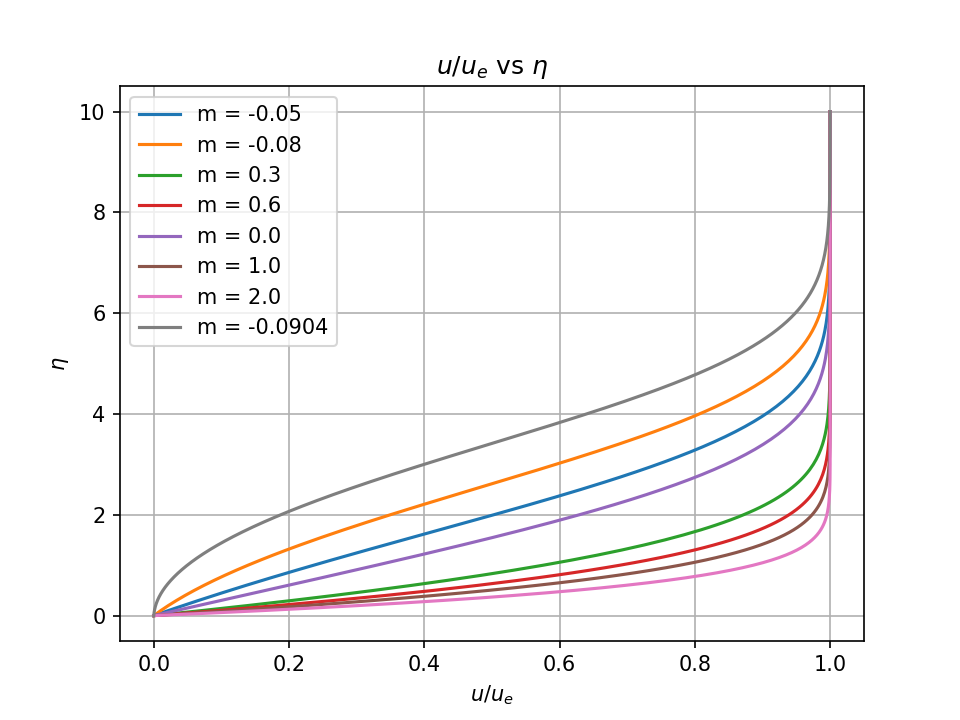
\includegraphics[scale=0.5]{supporting_documents/02_question_2_and_3_codeDevelopment/03_postProcessing/plot_1.png}
    \caption{streamwise velocity profiles plot for different m values}
    \label{plot_1}
\end{figure}

\par The streamwise velocity profile variations for different m values can
be found in \Cref{plot_1}. From the graph, it can be seen that as the
m value increases, the gradient of velocity is also increased. The velocity
profile for $m = -0.09043$ shows, the edge of separation.


\begin{figure}[!h]
   \centering
    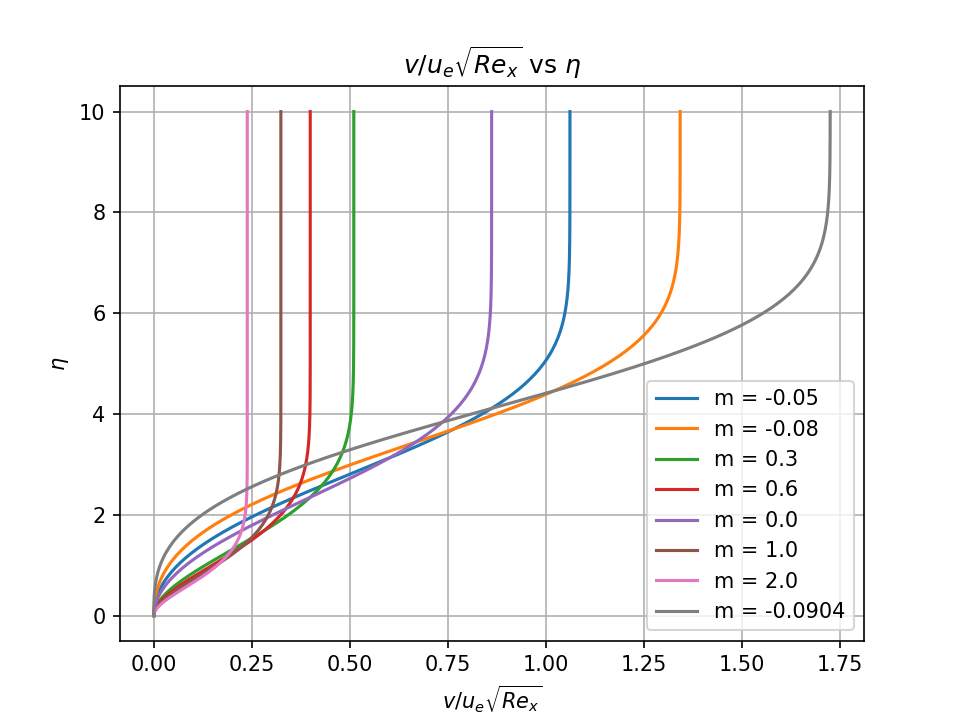
\includegraphics[scale=0.5]{supporting_documents/02_question_2_and_3_codeDevelopment/03_postProcessing/plot_2.png}
    \caption{normal velocity profiles plot for different m values}
    \label{plot_2}
\end{figure}

\par The normal velocity profiles given in \Cref{plot_2} for different m values
show that the normal velocity decreases with increase in m value, indicating
the change in wedge angle for the given flow.\\

\begin{figure}[!h]
   \centering
    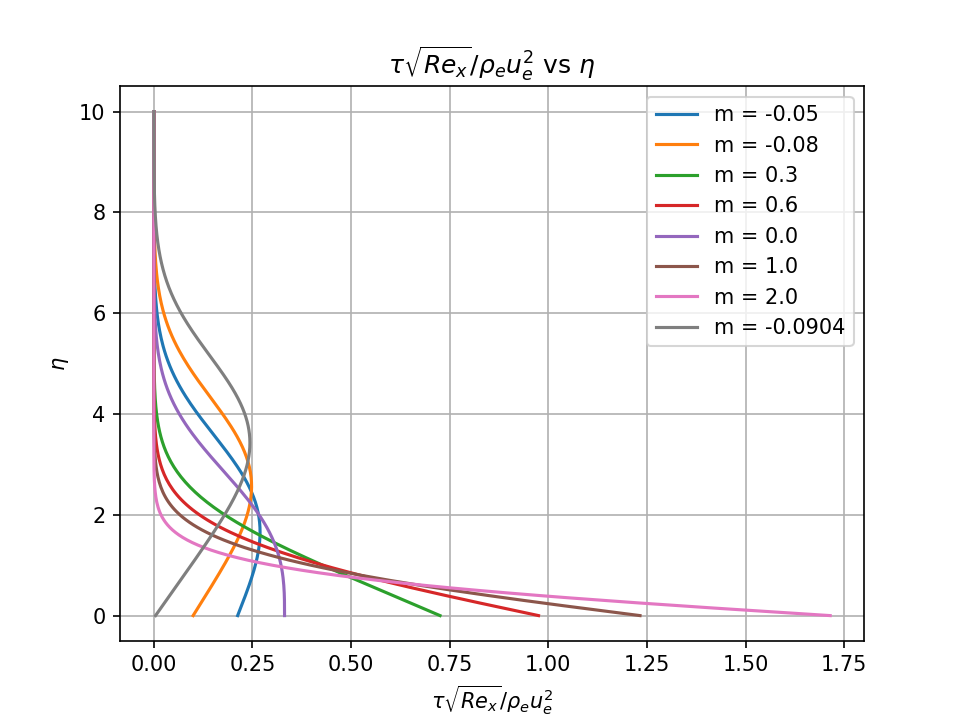
\includegraphics[scale=0.5]{supporting_documents/02_question_2_and_3_codeDevelopment/03_postProcessing/plot_3.png}
    \caption{shear stress profiles for different values of m}
    \label{plot_3}
\end{figure}

\par The shear stress profiles given in \Cref{plot_3} show the inflection of
profile for the m values less than 0, indicating a favourable shear stress
gradient for the flow, till the point of separation where the adverse pressure
gradient dominates the shear stress gradient.

\pagebreak

\subsection{Table of derived variables}

\par In this section, the computed variables i.e. $f$, $f^{\prime}$, $f^{\prime\prime}$, $f^{\prime\prime\prime}$
were used in obtaining values for derived variables given below.\\

\(\frac{\delta^*}{\delta_{FS}}\): \\
This parameter gives the nondimensional displacement thickness for the given
flow field. The value for this is obtained from solution variables as given
in \Cref{d_star_dFS}.
\begin{align}
    \delta^* &= \int{}{} \left(1 - \frac{u}{u_e}\right) dy \nonumber \\
    \frac{\delta^*}{\delta_{FS}} &= \int{}{}\left( 1 - f^{\prime}\right) d\eta \nonumber \\
    \frac{\delta^*}{\delta_{FS}} &= \left[\eta - f(\eta)\right]_0^{\eta_{max}} \label{d_star_dFS}
\end{align}

\par Similarly, the nondimensional momentum thickness is obtained by integration
and is given by \Cref{theta_dFS} and this has been solved by numerical integration.
\begin{align}
    \frac{\theta}{\delta_{FS}} &= \int{}{}\left(f^{\prime} - \left(f^\prime\right)^2\right)d\eta \label{theta_dFS}
\end{align}

\par And the nondimensional shearstress is obtained as \Cref{Rex_Cf}.
\begin{align}
    \tau &= \mu \frac{\partial u}{\partial y} \nonumber \\
    &= \mu u_e f^{\prime\prime}(\eta) \sqrt{\frac{u_e}{\nu x}} \nonumber \\
    \frac{\tau \sqrt{Re_x}}{\rho_e u_e^2} &= f^{\prime\prime}(\eta) \nonumber \\
    \frac{1}{2}C_f \sqrt{Re_x} &= f^{\prime\prime}(\eta)|_{@wall} \label{Rex_Cf}
\end{align}

\par The expressions for $\lambda$ and $\tau$ are given in \Cref{lambda,Tau}.
\begin{align}
    \lambda &= \frac{\theta^2}{\nu} \frac{d u_e}{dx} = m \left(\frac{\theta}{\delta_{FS}}\right)^2 \label{lambda} \\
    \tau &= Re_{\theta}\frac{C_f}{2} = \left(\frac{\theta}{\delta_{FS}}\right)^2 f^{\prime\prime} \label{Tau}
\end{align}

\par The values obtained for above variabeles for each m value are given in \Cref{table_f}. And
their comparison plots were given in \Cref{FS_numerical_plot}, the computed data
were compared against the book data given in \cite{ref_2} to show the
accuracy of computation.

\begin{table}
   \centering
    \caption{Falkner-Skan Equation's derived solution variables}
    \label{table_f}
    \begin{tabular}{|c|c|c|c|c|c|c|c|}
    \hline
        m & $\frac{\delta^*}{\delta_{FS}}$ & $\frac{\theta}{\delta_{FS}}$ & H & $\sqrt{Re_x}\frac{C_f}{2}$ & $\lambda$ & $\tau$ & $F_\theta$ \\ \hline
    -0.0904 & 3.45079 & 0.86796 & 3.97577 & 0.00433 & -0.0681 & 0.00376 & 0.82145 \\ \hline
    -0.08 & 2.68541 & 0.83128 & 3.23047 & 0.09964 & -0.05528 & 0.08283 & 0.74395 \\ \hline
    -0.05 & 2.12304 & 0.75256 & 2.82108 & 0.21247 & -0.02832 & 0.15989 & 0.59283 \\ \hline
    0.0 & 1.72351 & 0.66485 & 2.59233 & 0.33138 & 0.0 & 0.22032 & 0.44064 \\ \hline
    0.3 & 1.02025 & 0.44203 & 2.30809 & 0.72548 & 0.05862 & 0.32069 & 0.13631 \\ \hline
    0.6 & 0.79799 & 0.35472 & 2.24962 & 0.97514 & 0.0755 & 0.3459 & 0.05015 \\ \hline
    1.0 & 0.64822 & 0.29212 & 2.21902 & 1.23239 & 0.08533 & 0.36 & -4e-05 \\ \hline
    2.0 & 0.47682 & 0.21739 & 2.19343 & 1.71443 & 0.09451 & 0.37269 & -0.04728 \\ \hline
    \end{tabular}
\end{table}

\begin{figure}[!h]
    \begin{subfigure}{0.45\linewidth}
       \centering
        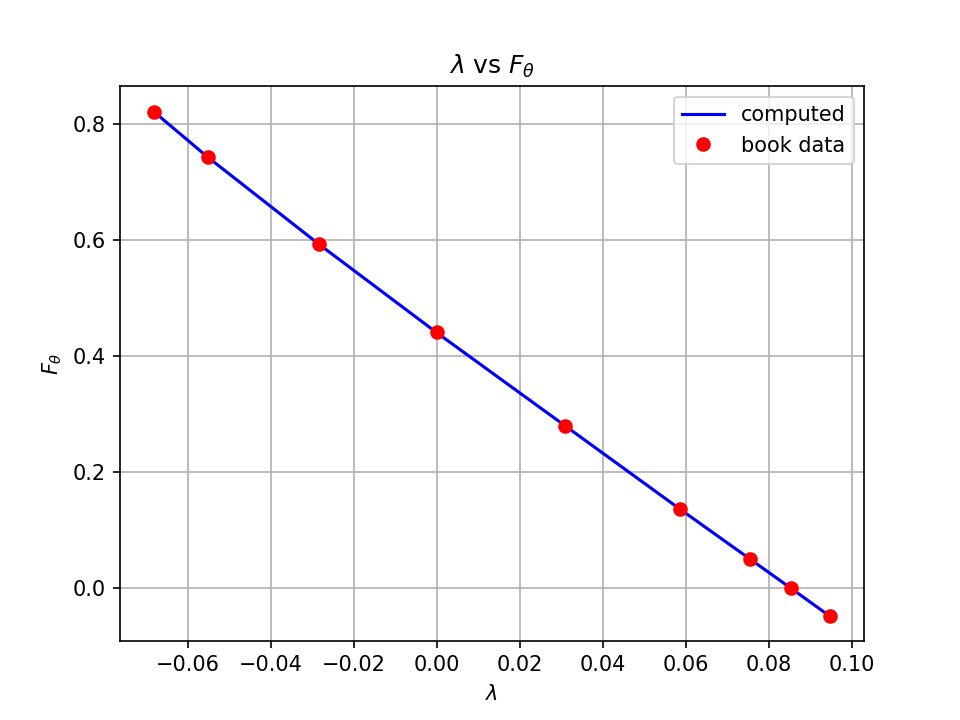
\includegraphics[scale=0.5]{supporting_documents/02_question_2_and_3_codeDevelopment/03_postProcessing/lambda_vs_F_theta.png}
        \caption{$\lambda$ vs $F_\theta$}
    \end{subfigure}
    \hfill
    \begin{subfigure}{0.45\linewidth}
       \centering
        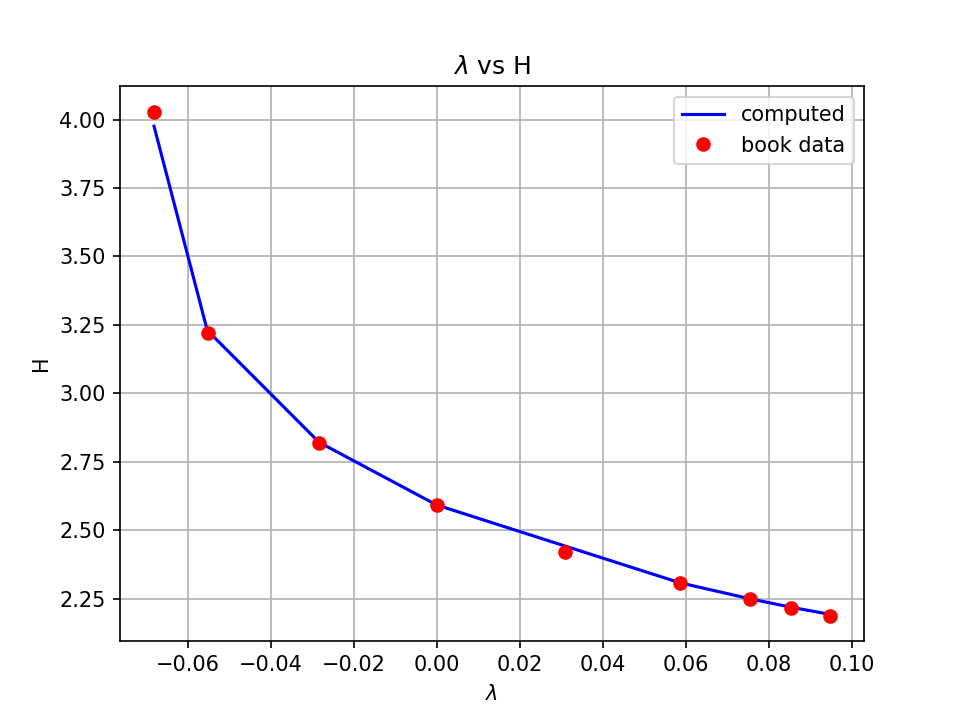
\includegraphics[scale=0.5]{supporting_documents/02_question_2_and_3_codeDevelopment/03_postProcessing/lambda_vs_H.png}
        \caption{$\lambda$ vs H}
    \end{subfigure}
    \hfill
    \begin{subfigure}{1.00\linewidth}
       \centering
        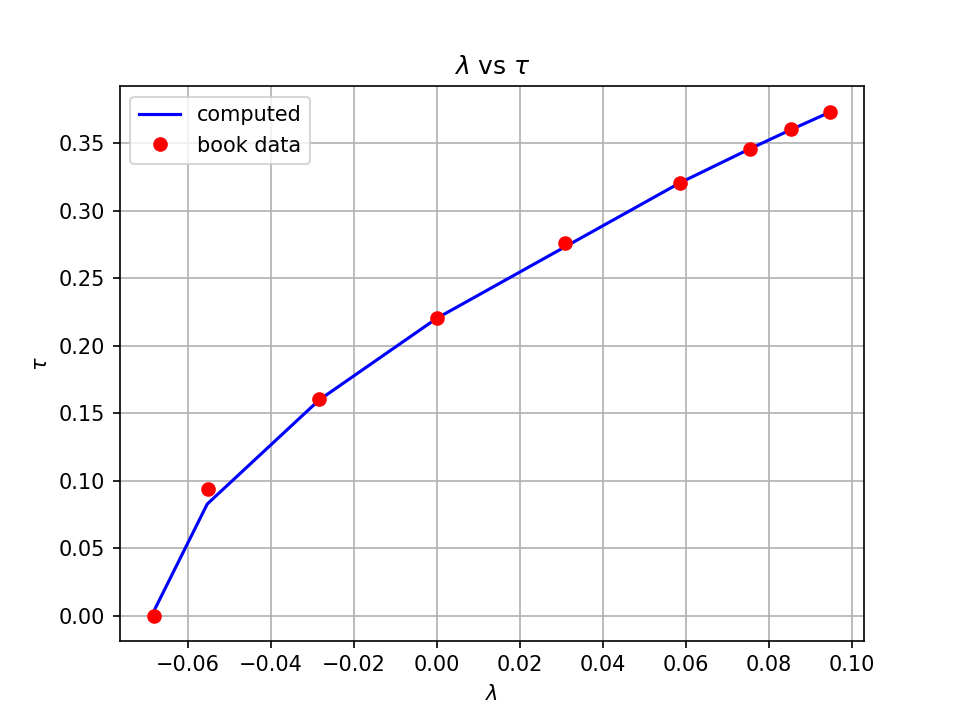
\includegraphics[scale=0.5]{supporting_documents/02_question_2_and_3_codeDevelopment/03_postProcessing/lambda_vs_Tau.png}
        \caption{$\lambda$ vs $\tau$}
    \end{subfigure}
    \caption{Variation of derived parameters vs $\lambda$}
    \label{FS_numerical_plot}
\end{figure}


\section{Question 3}
Calculate the value of \(\frac{\delta^*}{\delta_{FS}}, \frac{\theta}{\delta_{FS}}$,H,$\sqrt{Re_x}\frac{C_f}{2}$, fro the given
values of m using analytical Thwaits method and compare with the numerical solution of Falkner Skan equation.

\vspace{0.5cm}
\textbf{SOLUTION}
\vspace{0.5cm}

\par The procedure followed for computing given variables using Thwait's method is
given below.\\

\par The given velocity profile is assumed to be governed by power-law, i.e., $u_e(x) = A x^m$ \\

\par Then the following equation is used to compute the momentum thickness
from the velocity profile.
\begin{align*}
    \frac{\theta^2}{\nu} &= \frac{0.45}{u_e^6}\int{}{}u_e^5 dx \\
    \frac{\theta^2}{\nu} &= \frac{0.45 x^{1-m}}{A \left(5m+1\right)}
\end{align*}

\par The nondimensional distance parameter $\lambda$ is then calculated as follows.

\begin{align*}
    \lambda &= \frac{\theta^2}{\nu} \frac{d u_e}{dx} \\
            &= \frac{0.45 m}{5 m + 1}
\end{align*}

\par Then, the values of $H$ and $T$ are computed using the given approximate
expression as
\begin{align*}
    H(\lambda) &= 2.62 - 4.1 \lambda + 14 \lambda^3 + \frac{0.56\lambda^2}{(\lambda+0.18)^2} \\
    T(\lambda) &= 0.22 + 1.52 \lambda - 5 \lambda^3 - \frac{0.072 \lambda^2}{(\lambda + 0.18)^2}
\end{align*}

\par Using, the values of $H$ and $T$ computed above, the following values
were computed.
\begin{align*}
    H &= \frac{\delta^*}{\theta} \rightarrow \delta^* = H \theta \\
    \frac{\delta*}{\delta_{FS}} &= H \sqrt{\frac{0.45}{5m+1}} \\
    \frac{\theta}{\delta_{FS}} &= \sqrt{\frac{0.45}{5m+1}}
\end{align*}

\par Lastly, the nondimensional shear stress is computed as follows.
\begin{align*}
    \tau &= Re_\theta \frac{C_f}{2} \rightarrow \sqrt{Re_x}\frac{C_f}{2} = \frac{T}{\left(\frac{\theta}{\delta_{FS}}\right)}
\end{align*}

\par The computed analytical values were compared with the above computed
numerical values in \Cref{plot_a_1,plot_a_2,plot_a_3,plot_a_4,plot_a_5}. \\

\begin{figure}
   \centering
    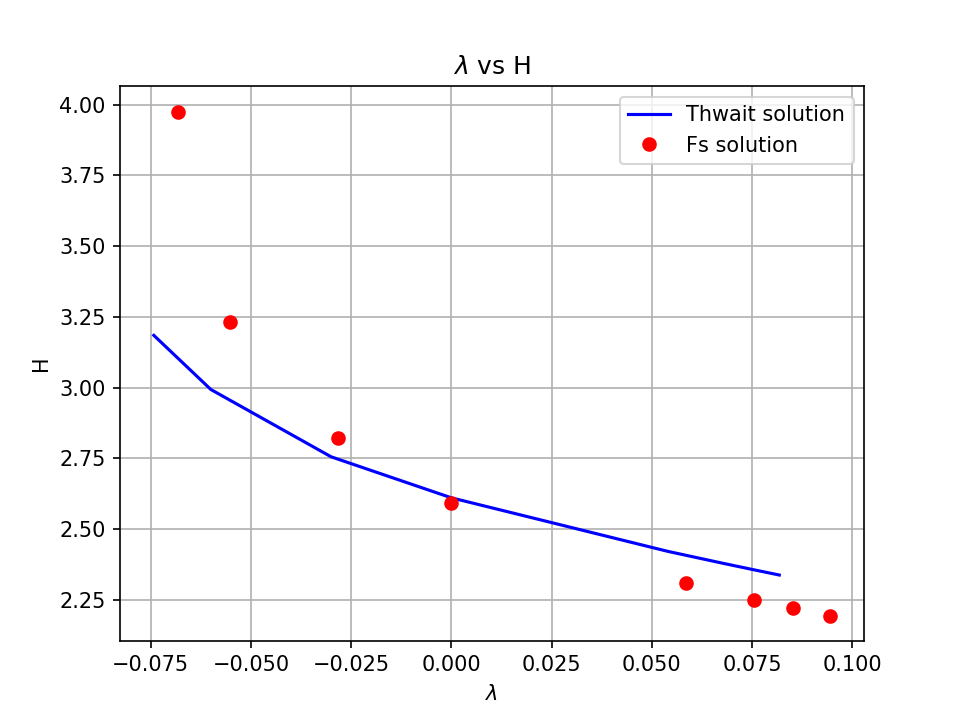
\includegraphics[scale=0.5]{supporting_documents/02_question_2_and_3_codeDevelopment/03_postProcessing/lambda_vs_H_thwait.png}
    \caption{ $\lambda$ vs $H$}
    \label{plot_a_1}
\end{figure}

\begin{figure}
   \centering
    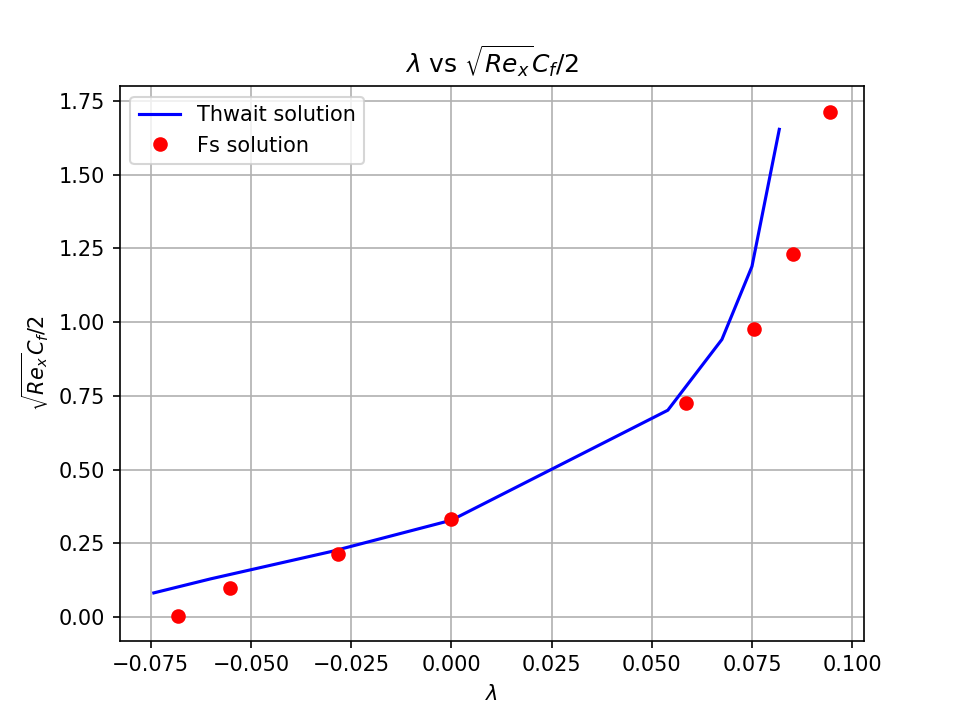
\includegraphics[scale=0.5]{supporting_documents/02_question_2_and_3_codeDevelopment/03_postProcessing/lambda_vs_Rex_Cf_thwait.png}
    \caption{ $\lambda$ vs $\sqrt{Re_x}\frac{C_f}{2}$}
    \label{plot_a_2}
\end{figure}

\begin{figure}
   \centering
    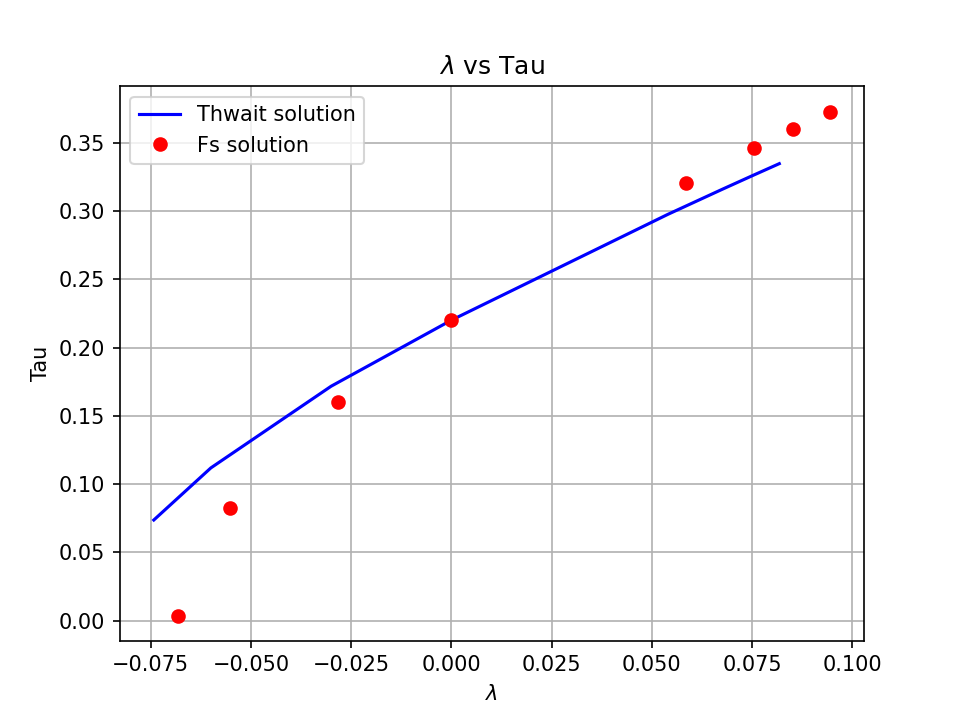
\includegraphics[scale=0.5]{supporting_documents/02_question_2_and_3_codeDevelopment/03_postProcessing/lambda_vs_Tau_thwait.png}
    \caption{ $\lambda$ vs $T$}
    \label{plot_a_3}
\end{figure}

\begin{figure}
   \centering
    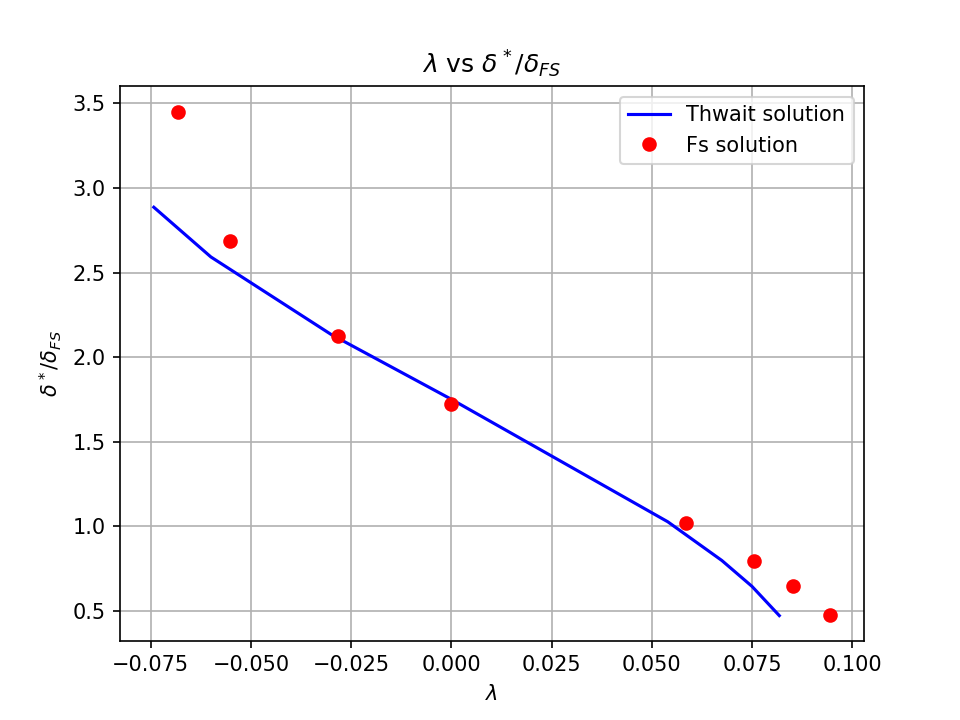
\includegraphics[scale=0.5]{supporting_documents/02_question_2_and_3_codeDevelopment/03_postProcessing/lambda_vs_d_star_dFS_thwait.png}
    \caption{ $\lambda$ vs $\frac{\delta^*}{\delta_{FS}}$ }
    \label{plot_a_4}
\end{figure}

\begin{figure}
   \centering
    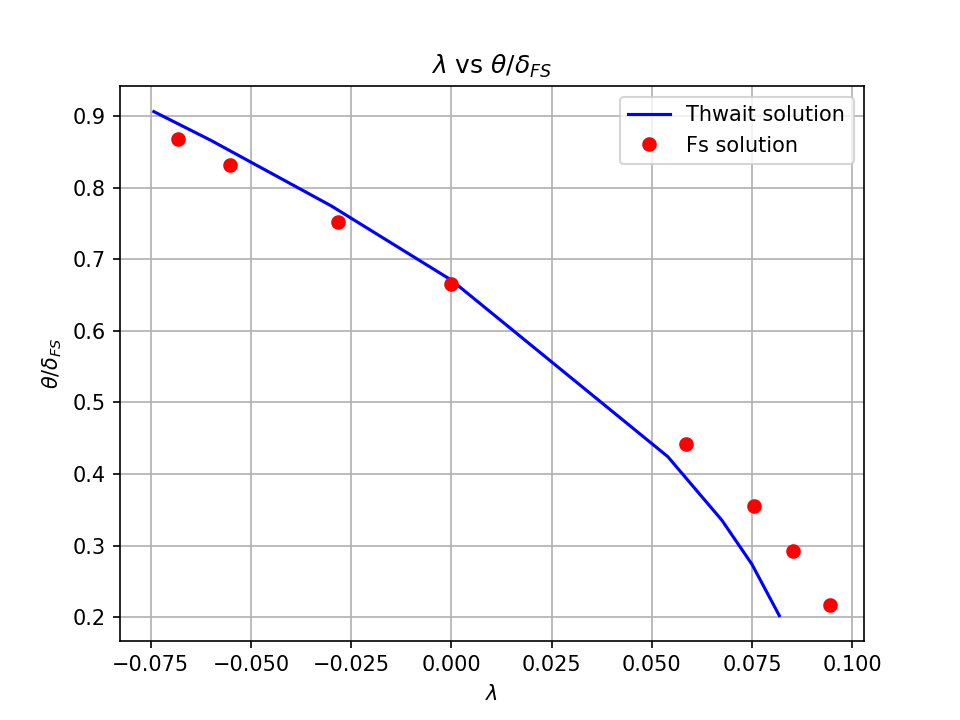
\includegraphics[scale=0.5]{supporting_documents/02_question_2_and_3_codeDevelopment/03_postProcessing/lambda_vs_theta_dFS_thwait.png}
    \caption{ $\lambda$ vs $\frac{\theta}{\delta_{FS}}$}
    \label{plot_a_5}
\end{figure}

\par It can be seen that the Thwait solution does not match well with the
numerical solution, but it is sufficient enough for the preliminary
computations. The \emph{Python} code developed for this post-processing
is given in \Cref{pp_code}.

\pagebreak


\begin{thebibliography}{2}
    \bibitem{ref_1}  Han, S. "Finite Difference Solution of the Falkner—Skan Wedge Flow Equation." International Journal of Mechanical Engineering Education 41.1 (2013): 1-7.
    \bibitem{ref_2} Drela, Mark. Flight vehicle aerodynamics. MIT press, 2014.

\end{thebibliography}

\pagebreak

\begin{appendices}

    \section{Appendix - Finite Difference Method code for FS equation}\label{FDM_code}
    This section contains the Python code that solves the FS equation using
    Finite Difference Method.
    \lstinputlisting[language=python]{supporting_documents/02_question_2_and_3_codeDevelopment/01_FDM/script_FDM.py}

    \section{Appendix - Shooting Method code for FS equation}\label{SH_code}
    This section contains the Python code that solves the FS equation using
    Shooting Method.
    \lstinputlisting[language=python]{supporting_documents/02_question_2_and_3_codeDevelopment/02_shootingMethod/script_SM.py}

    \section{Appendix - Post-processing code}\label{pp_code}
    This section contains the Python code that is used for postProcessing the computed data.
    \lstinputlisting[language=python]{supporting_documents/02_question_2_and_3_codeDevelopment/03_postProcessing/script_processing.py}

\end{appendices}

\par
\center{**********}

\end{document}
